\newpage
\section{Durchführung}
Der Aufbau des Michaelson Interferometers ist in \autoref{fig:1} dargestellt. 

\begin{figure}
    \centering
    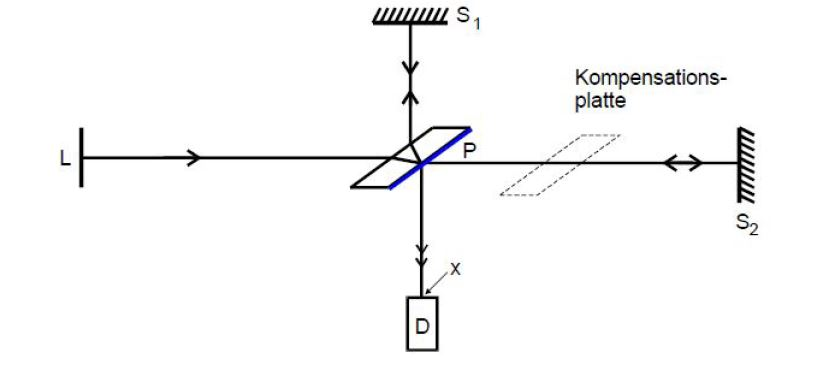
\includegraphics[scale = 0.7]{Picture/Pic1.JPG}
    \caption{Aufbau eines Michelson-Interferometers.
            Mit Lichtquelle = $L$, dem Strahlenteiler = $P$, den Spiegel $S_1$ und $S_2$, dem semipermeabler Spiegel $P$ und dem Detektor $D$}
    \label{fig:1}
  \end{figure}

Zunächst muss der Aufbau so eingestellt werden, dass die beiden hellsten Punkte sich genau auf der Detektor
Öffnung überschneiden. Jedoch muss, damit die Koherenz des Lichtes nicht verletzt wird, der Wegunterschied zwischen den beiden Strahlenwegen kleiner als die Koherenzlänge 
\begin{equation*}
    l = n \lambda
  \end{equation*}
\noindent
sein. Dies wird dardurch realisiert, dass für die Abstände 
\begin{equation*}
    \overline{S_1 P} \approx \overline{S_2 P}
    \label{eqn:close}
\end{equation*}
\noindent
gilt. Wenn der Zusammenhang $\overline{S_1 P} = \overline{S_2 P}$ erfüllt ist kommt es zur destruktiven Interferenz. Zusätzlich ist eine Kompensationsplatte in dem Arm eingebaut, 
inwelchem der transmittierte Strahl unterwegs ist, da dieser zweimal weniger den Strahlenteiler $P$ durchläuft als der reflektierte. Dies wird durch die Kompensationsplatte ausgeglichen.
\noindent


\subsection{Wellenlängenmessung}
Um die Wellenlänge des Lasers experimentell zu bestimmen, wird mithilfe eines hoch ubersetzten Motor eine Mikrometerschraube gesteuert, welche durch einen Übersetzungsarm mit dem 
Spiegel $S_1$ verbunden ist. Durch die Drehung der Schraube kann der Spiegel um die Srecke $\symup{\Delta} d$ verschoben werden. Um genaue Ergebnisse zu erhalten werden ungefähr 
3000 auftretende Interferenzringe gemessen. 
Um die Wellenlänge zu bestimmen wird der Zusammenhang
\begin{equation*}
    \symup{\Delta}d = \frac{z \cdot \lambda}{2}
    \label{eqn:d2}
\end{equation*}
\noindent
genutzt. 

\subsection{Brechungsindex Bestimmung}
Für die Messung des Brechungsindexes wird der Versuchsaufbau etwas umgeändert. Dies ist in Abbildung \ref{fig:2} zu sehen.

\begin{figure}
    \centering
    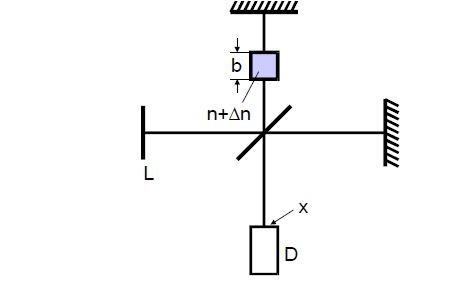
\includegraphics[scale = 0.7]{Picture/Pic2.JPG}
    \caption{Aufbau des Michelson-Interferometers mit Abschnitt der Länge $b$ und des
    Brechungsindizes $n + \symup{\Delta}n$ auf der Strecke $\overline{S_1 P}$}
    \label{fig:2}
  \end{figure}
\noindent
Durch variation des Drucks über die Strecke $b$ durch eine Vakuumkammer, kann ein Wegunterschied zwiscen den Strahlenbündeln von $\symup{\Delta}nb$ gemessen werden. Somit 
gilt mit der vorherigen Überlegung

\begin{equation*}
    \symup{\Delta}nb = \frac{z \cdot \lambda}{2} \; .
    \label{eqn:nb2}
  \end{equation*}

Zusätzlich gilt für den Brechungsindex $n$ 
\begin{equation*}
  n(p_0, T_0) = 1 + \symup{\Delta} n (p,p') \frac{T}{T_0} \frac{p_0}{p - p'} \; .
  \label{eqn:brech}
\end{equation*}

